\documentclass[11pt,mathserif]{beamer}


%% ====== packages ==
\usepackage{amsmath,amssymb,amsfonts,amsthm}
\usepackage{graphicx}
\newcommand{\tiret}{\rule[0.6ex]{1.3ex}{0.22ex}}

% !! pour le francais
\usepackage[utf8]{inputenc}
\usepackage[french]{babel}
\usepackage{fancyvrb}
%\usepackage{verbatim}
\usepackage{relsize}
\usepackage{color}
\usepackage{listings}


\newcommand{\R}{\mathbb{R}}


% et la commande Pour les guillemets
\newcommand{\guill}[1]{«#1»} % attention deja dans mycv


%% ====== my bearmer ==
\mode<presentation> {
\usetheme{default}    % sobre

% options
\useinnertheme[shadow]{rounded}  % les numeros
}
\usefonttheme{structurebold}

\begin{document}

%****************************************************************
% Page de presentation 
%**************************************************************
\begin{frame}
\begin{center}
{\Large Une introduction au calcul sur GPU} 
\end{center}
\begin{center}
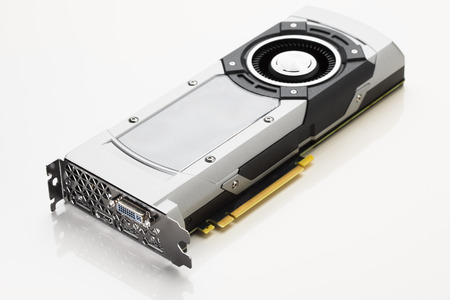
\includegraphics[width=0.5\linewidth]{gpu.jpg}
\end{center}
\begin{center}
{\large Marc Fuentes - INRIA \\ }
\end{center}
\end{frame}

%****************************************************************
% Plan
%**************************************************************

\begin{frame}
\frametitle{Plan}

\begin{itemize}[<+->]
\item Prolégomenes( parallèlisme, mémoire, cache)
\item Architecture des GPU
\item CUDA
\end{itemize}
\end{frame}

%****************************************************************
% Prolegomènes I
%****************************************************************
\begin{frame}
\frametitle{Parallèlisme}
\pause
différentes classifications du parallèlisme
\begin{itemize}[<+->]
  \item partagé / distribué
    \begin{itemize}
      \item à mémoire partagée : OpenMP, fils d'éxecution, GPU (partiellement)
      \item à mémoire distribué : MPI
    \end{itemize}
 \item gros grain / grain fin : taille des tâches
   \begin{itemize}
     \item gros grain : MPI, certains tâches en mémoire partagée
     \item grain fin : noyau GPU s'executant sur beaucoup de cœurs
   \end{itemize}
 \item homogène / hétérogène 
   \begin{itemize}
     \item archi homogène : MPI, processeur vectoriels
     \item hétérogène : GPU(accélérateur) et CPU(hôte) , processeur Cell 
   \end{itemize}
\end{itemize}
\pause
$\Rightarrow$ La programmation sur GPU est donc un parallèlisme à grain fin à mémoire partagée avec une architecture hétérogène. Elle va
donc bien convenir à certains types de problèmes
\end{frame}

%****************************************************************
% Prolègomène II
%****************************************************************
\begin{frame}{Mémoire et Cache}
\begin{itemize}[<+->]
  \item La rapidité d'execution d'un calcul dépend aussi de la «proximité» avec le CPU de l'élément de mémoire à traiter 
  \item si $l$ represente la latence - en nombre de cycle d'horloge - de l'emplacement mémoire accèdé
  $$l({\mbox{\scriptsize registre}}) \leqslant l(\mbox{\scriptsize cache L1}) \leqslant
    l(\mbox{\scriptsize cache L2}) \leqslant l(\mbox{\scriptsize mémoire globale})$$
  \item exemple pour un Core i7 Xeon
    \begin{tabular}{|l|c|c|}
    \hline
      type & nb cycles & latence (ns)  \\
    \hline
      cache L1  & $\approx$ 4 & 2.1 - 1.2 \\
      cache L2  & $\approx$ 10 & 5.3 - 3.0ns \\
      cache L3 (non partagé)  & $\approx$ 40 & 21.4 - 12ns \\
    \hline
    \end{tabular}

  \item les architectes de CPU ont crée des caches pour stocker les valeurs mémoires les plus utilisées
\end{itemize}
\begin{center}
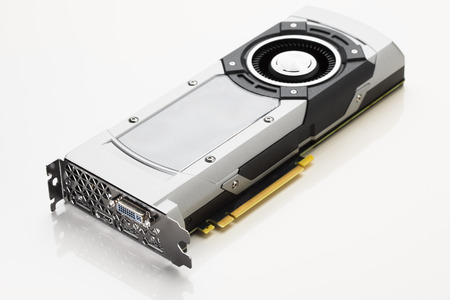
\includegraphics[width=0.5\linewidth]{gpu.jpg}
\end{center}
\end{frame}
%****************************************************************
%% Epetra Maps 
%%****************************************************************
%\begin{frame}{Epetra : Maps I}
%\begin{itemize}[<+->]
%\item Comment répartir un objet sur plusieurs processus MPI ?
%\item Notion de correspondance (\guill{Map}) : on utilise un tableau d'indices qui indique quelles composantes sont situées sur quel proc.
%\item soit le programme suivant :
%\fvset{fontsize=\relsize{-3}}
%\lstinputlisting[language=python]{prog1.py}
%\item que l'on lance avec la commande suivante : \Verb+mpiexec -n 2 xterm -e ./prog1.py+
%\end{itemize}
%\end{frame}
%%****************************************************************
%% Epetra  Maps II
%%****************************************************************
%\begin{frame}{Epetra : Maps II}
%\begin{center}
%on obtient les sorties suivantes:
%\end{center}
%\begin{minipage}[c]{0.49\linewidth}
%\fvset{fontsize=\relsize{-3}}
%\VerbatimInput{sortie1}
%\end{minipage}
%\begin{minipage}[c]{0.49\linewidth}
%\fvset{fontsize=\relsize{-3}}
%\VerbatimInput{sortie2}
%\end{minipage}
%\end{frame}
%%****************************************************************
%% Epetra  Maps II
%%****************************************************************
%\begin{frame}{Epetra : Maps III}
%\begin{itemize}[<+->]
%\item chaque processus a donc un ensemble d'indices disponibles
%\item on a l'isomorphisme 
%\fvset{fontsize=\relsize{-3}}
%$$
%  \{\mbox{indices locaux }\} \begin{array}{c} \buildrel \mbox{\Verb+Map.GID+} \over \longrightarrow \\ \buildrel \mbox{\Verb+Map.LID+} \over \longleftarrow \end{array} \{\mbox{indices globaux}\}
%$$
%\item la répartition sur les processeurs peut etre : automatique ou choisie : 
%      \begin{itemize} 
%       \item automatique : constructeur \lstinline! __init__(self, int numGlobalElements, int indexBase, Comm comm)! \\ avec \lstinline! numGlobalElements=-1!
%       \item choisie selon le proc : constructeur \lstinline !__init__(self, int numGlobalElements, PySequence myGlobalElements, int indexBase, Comm comm)!
%    
%      \end{itemize}
%\end{itemize}
%\end{frame}
%%****************************************************************
%% Epetra : matrices 
%%****************************************************************
%\begin{frame}{Epetra : matrices}
%\begin{itemize}[<+->]
%\item \textcolor{red}{problème} : approche précédente valide seulement pour le 1D ! comment on généralise
%pour les matrices
%\item \textcolor{blue}{solution} : Trilinos généralise au cas matriciel, en associant deux  {\bf correspondances} à 
%une matrice donnée. Ainsi pour une matrice au format CRS (Compressed Row Storage), on a 
%    \begin{itemize}
%       \item un découpage en colonnes : \lstinline! CrsMatrix.DomainMap!  
%       \item un découpage en ligne : \lstinline! CrsMatrix.RangeMap!  
%    \end{itemize}
%\item l'utilisateur peut a priori agir sur ces deux correspondances, mais c'est parfois plus simple
%de laisser PyTrilinos organiser le découpage en fonction des valeurs non-nulles de la matrice
%\end{itemize}
%\end{frame}
%%****************************************************************
%% Exemple : gradient conjugue
%%****************************************************************
%\begin{frame}{Exemple : gradient conjugué}
%\begin{itemize}[<+->]
%\item On considère une version naïve de l'algorithme du gradient conjugué : 
%\end{itemize}
%\pause
%\begin{center}
%\begin{algorithmic}[1]
%\State $r \gets b - A x_0$
%\State $p \gets r$
%\State $\rho \gets \prods{r}{r}$
%\While{$\sqrt{\rho} \geqslant \varepsilon \|F\|$}
%   \State $ \alpha \gets \frac{\|r\|}{\prods{p}{A p}}$
%   \State $ x \gets x + \alpha  p$
%   \State $ r \gets r - \alpha A p$
%   \State $ \rho_{+} \gets \prods{r}{r} $ 
%   \State $p \gets r + \frac{\rho_{+}}{\rho} p$
%   \State $\rho \gets \rho_{+}$
%\EndWhile
%\end{algorithmic}
%\end{center}
%\end{frame}
%%****************************************************************
%% Exemple : gradient conjugue
%%****************************************************************
%\begin{frame}{Exemple : gradient conjugué}
%\begin{center}
%On code 2 versions : MALAB vs PyTrilinos   
%\end{center}
%\begin{minipage}[c]{0.49\linewidth}
%\lstinputlisting[language=matlab]{mycg.m}
%\end{minipage}
%\begin{minipage}[c]{0.49\linewidth}
%\lstinputlisting[language=python]{EpetraCG.py}
%\end{minipage}
%\end{frame}
%%****************************************************************
%% Exemple : Running  
%%****************************************************************
%\begin{frame}{Performance du gradient conjugué}
%\begin{itemize}[<+->]
% \item On utilise l'algorithme suivant sur une matrice du laplacien-3d ( 
% $n = 10^{6}$, $nnz = 6940000$) avec $x_0(:) = 1$, $y(:) = 1$, 
% $\epsilon = 10^{-6}$, on converge en 201 iterations avec un résidu de $9.2 10^{-4}$
% \item on a code une version malab du cg, et on lance sur dantxaria (plafrim, héhé) le code Python pour différents nombres de procs :  
% \Verb+mpirun -np n python test\_CG.py+
% \item on chronométre uniquement l'algo de cg
%\end{itemize}
%\pause
%\begin{tabular}{|l||c|c|c|c|c|c||c|}
%\hline
%\#CPUs & 1 & 2 & 4 & 10 & 20 & 40 & MALAB  \\
%\hline
%tps(s) & 7.36  & 5.88 &  5.41 & 2.78 & 1.84 & 1.44 & 13.74 \\
%\hline
%\end{tabular}
%\end{frame}

\end{document}
